
\section{Study Dataset}

We select the simulation results and validation analysis done by \citet{Taborda_2014_BSSA} as our reference dataset, hereafter the dataset. In that study, the authors carried out deterministic simulations for the 2008 \eqmag{w} 5.4 Chino Hills, California, earthquake using a finite-element approach. The simulations, done for a kinematic finite-fault model of the earthquake, were computed for a maximum frequency \fmaxeq{4} and a minimum shear wave velocity \vsmineq{200}. In total, \citet{Taborda_2014_BSSA} did three simulations, each for a different velocity model \citep[CVM-S4, CVM-H, CVM-H+GTL, see][]{Small_2017_SRL}. The modeling domain covered an area of \adomain{180}{135}{km} that included all the major sedimentary basins and other relevant geologic structures in the greater Los Angeles region. Their validation analysis consisted of comparisons with data recorded during the event at 336 ground motion monitoring stations, for the three \change{components} of motion (EW, NS, and UD). The simulation domain and the stations used for the analysis are shown in Figure \ref{fig:chino-hills}, and a sample of the validation results obtained by \citet{Taborda_2014_BSSA} using \citeauthor{Anderson_2004_Proc}'s approach is shown in Figure \ref{fig:ref-gof-maps}. This second figure, in particular, shows the spatial distribution of GOF scores (interpolated from the values at each station) for the comparison of the broadband synthetics and data, averaged for all metrics, and the three \change{components} of motion.

\begin{figure*}[t]
    \centering
    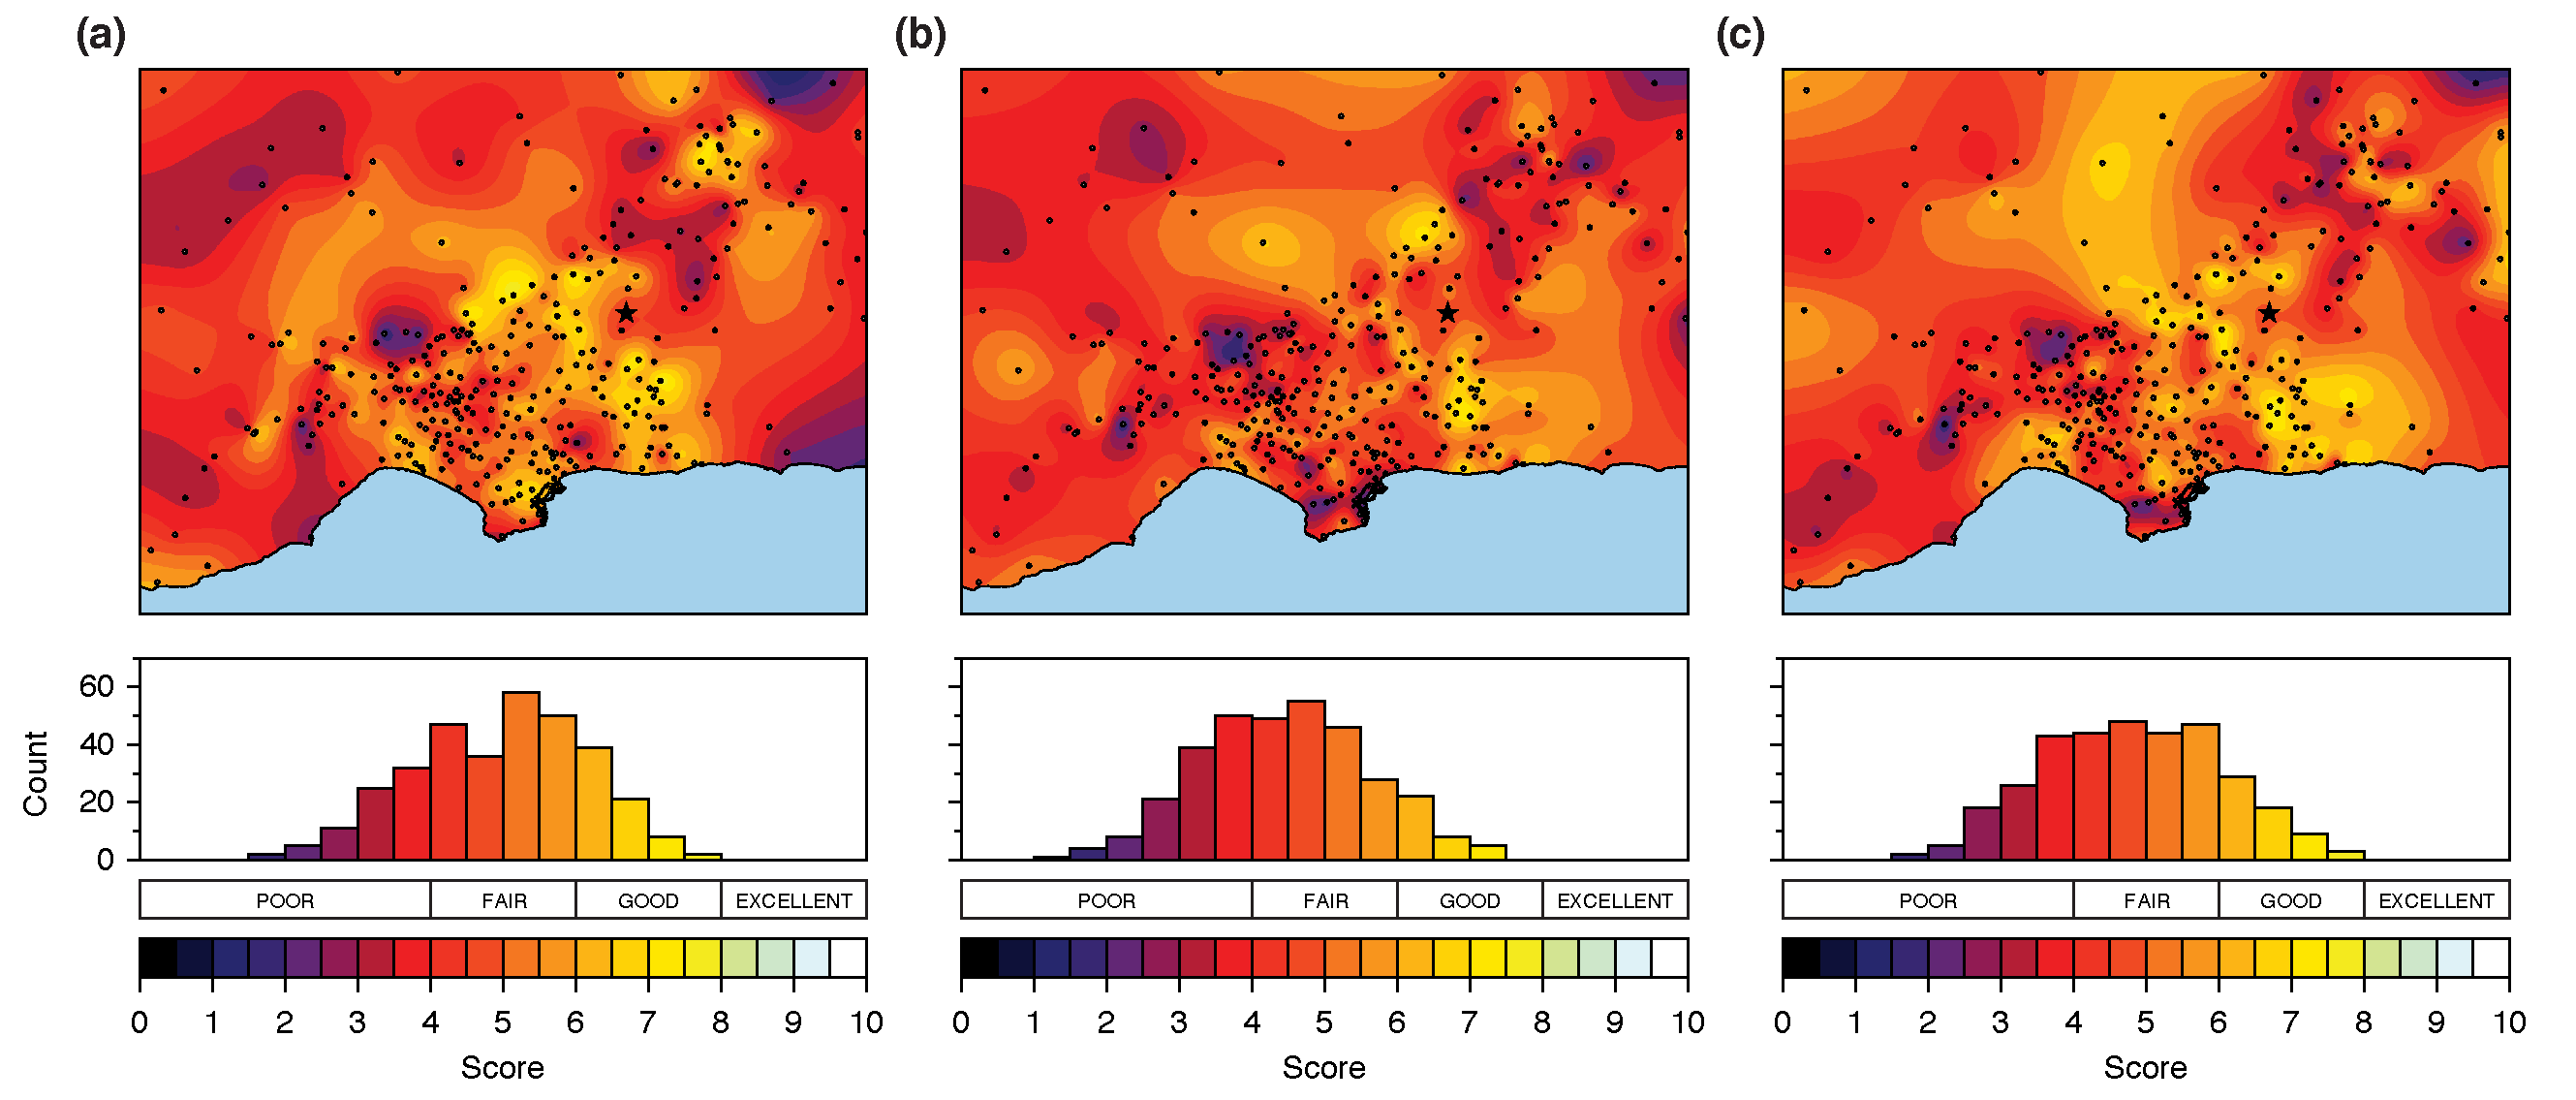
\includegraphics[width=\textwidth]{figures/pdf/figure-02}
    \caption{Validation results obtained by \citet{Taborda_2014_BSSA} in the form of GOF values across the region of interest obtained from comparisons between simulations for three different velocity models and data recorded at ground motion monitoring stations. The color version of this figure is available only in the electronic edition.}
    \label{fig:ref-gof-maps}
\end{figure*}
% 
\begin{figure}[ht!]
    \centering
    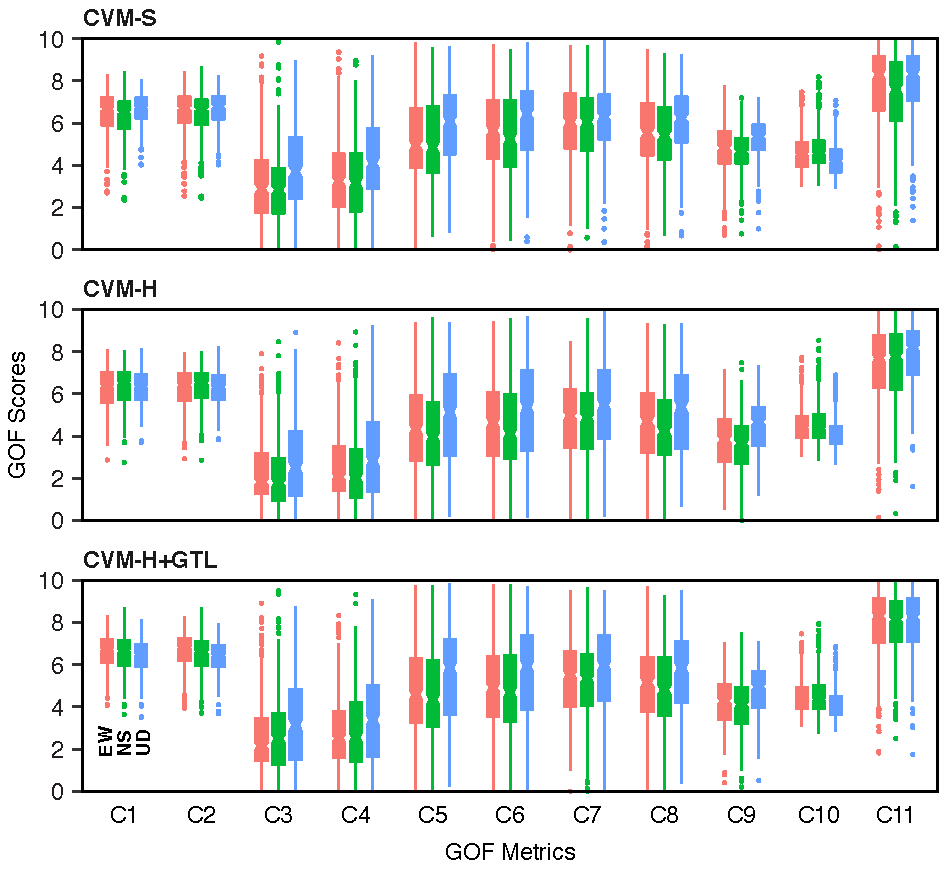
\includegraphics[width=0.48\textwidth]{figures/pdf/figure-03}
    \caption{Statistical distribution of the GOF dataset obtained from \citet{Taborda_2014_BSSA} shown in the form of box-plots for each metric (C1 through C11, see Table \ref{tab:metrics}), velocity model (CVM-S, CVM-H, and CVM-H+GTL), and \change{components of motion} (NS, EW, UD). In each case, \change{the boxes represent the interquartile range ($\mathrm{IQR} = \mathrm{Q}3 - \mathrm{Q}1$), the medians are indicated by a notch in the boxes, and the vertical lines show} the range of the data, with outliers (data less than $\mathrm{Q}1 - 1.5 \mathrm{IQR}$ and greater than $\mathrm{Q}3 + 1.5 \mathrm{IQR}$) shown as scattered dots. The color version of this figure is available only in the electronic edition.}
    \label{fig:data-box-plot}
\end{figure}

Here, we use the GOF scores obtained by \citet{Taborda_2014_BSSA} independently of the velocity models and/or the \change{components of motion}. Although at times we will make distinctions between the models and the components for visualization purposes, the clustering analysis to be described in the following section was done using the whole dataset of scores. The motivation behind this choice was that the dataset, as a sample of GOF values, was independent of the simulation and serves here as a generic set for the purpose of identifying the correlations that exist between the different metrics in Table \ref{tab:metrics}. As such, given the simulations for each velocity model (3), the motion components (3), and the number of stations used in the validation (336) gave us a large enough sample of 3,024 GOF scores. Figure \ref{fig:data-box-plot} illustrates this idea by comparing the statistical distribution of the broadband GOF scores of the simulations classified by velocity models and components. It is clear that although there are differences between them, these are negligible; in other words, the statistical distribution of results for each metric is about the same independently of model or component. Consequently, we combine all the data into a single dataset.
